% 
% Annual Cognitive Science Conference
% Sample LaTeX Paper -- Proceedings Format
% 

% Original : Ashwin Ram (ashwin@cc.gatech.edu)       04/01/1994
% Modified : Johanna Moore (jmoore@cs.pitt.edu)      03/17/1995
% Modified : David Noelle (noelle@ucsd.edu)          03/15/1996
% Modified : Pat Langley (langley@cs.stanford.edu)   01/26/1997
% Latex2e corrections by Ramin Charles Nakisa        01/28/1997 
% Modified : Tina Eliassi-Rad (eliassi@cs.wisc.edu)  01/31/1998
% Modified : Trisha Yannuzzi (trisha@ircs.upenn.edu) 12/28/1999 (in process)
% Modified : Mary Ellen Foster (M.E.Foster@ed.ac.uk) 12/11/2000
% Modified : Ken Forbus                              01/23/2004
% Modified : Eli M. Silk (esilk@pitt.edu)            05/24/2005
% Modified : Niels Taatgen (taatgen@cmu.edu)         10/24/2006
% Modified : David Noelle (dnoelle@ucmerced.edu)     11/19/2014
% Modified : Roger Levy (rplevy@mit.edu)     12/31/2018



%% Change "letterpaper" in the following line to "a4paper" if you must.

\documentclass[10pt,letterpaper]{article}

\usepackage{cogsci}

% \cogscifinalcopy % Uncomment this line for the final submission 


\usepackage{pslatex}
\usepackage{apacite}
\usepackage{float} % Roger Levy added this and changed figure/table
                   % placement to [H] for conformity to Word template,
                   % though floating tables and figures to top is
                   % still generally recommended!

%\usepackage[none]{hyphenat} % Sometimes it can be useful to turn off
%hyphenation for purposes such as spell checking of the resulting
%PDF.  Uncomment this block to turn off hyphenation.


%\setlength\titlebox{4.5cm}
% You can expand the titlebox if you need extra space
% to show all the authors. Please do not make the titlebox
% smaller than 4.5cm (the original size).
%%If you do, we reserve the right to require you to change it back in
%%the camera-ready version, which could interfere with the timely
%%appearance of your paper in the Proceedings.

% erikb new packages
\usepackage{graphicx}
\usepackage{color}
\newcommand{\eb}[1]{{\color{blue}{\bf\sf [EB: #1]}}}


\title{Trust in learning agents}
 
\author{{\large \bf Erik Brockbank (ebrockbank@ucsd.edu)} \\
  Department of Psychology, 9500 Gilman Drive \\
  La Jolla, CA 92093 USA
  \AND {\large \bf Judith Fan (jefan@ucsd.edu)} \\
  Department of Psychology, 9500 Gilman Drive \\
  La Jolla, CA 92093 USA}


\begin{document}

\maketitle


\begin{abstract}
ABSTRACT GOES HERE.

\textbf{Keywords:} 
trust; social inference
\end{abstract}


\section{Introduction}

\textit{How do people build up trust across repeated interactions?} This question has motivated research from diverse areas of cognitive science spanning social psychology [CITE], game theory and economics [CITE], and, as automated agents become increasingly ubiquitous in our everyday lives, robotics and human-computer interaction (HCI) [CITE]. 
In automated driving settings for instance, people routinely make decisions about how much to trust an artificial driving agent. And in many industrial domains, people work closely with automated agents, sometimes for high stakes tasks. The emergence of trust in our interactions with humans and artificial agents involves a range of complex social inferences, for example recognizing that one's collaborator shares one's goals or utilities to begin with [CITE]. However, one of the central features of human collaboration with artificial agents is that we trust them to be \textit{competent} across a range of task settings. Indeed, greater levels of trust may simply correspond to a belief that the agents are competent in a wider range of settings (e.g., greater trust in an autonomous vehicle may in large part reflect a belief that they can handle a wide array of driving environments and challenges).

Here we focus on the question of how people assess another agent's competence and how this affects downstream decisions about whether or not to trust them. Prior work in developmental psychology has shown that inferences about another person's competence based on their behavior emerge early in development and draw on a rich set of inputs. [EXAMPLES]. Broadly, this research suggests that when assessing another agent's competence, people bring a rich cognitive toolkit and a great deal of experience starting from a young age. Recent work in robotics and HCI suggests that when determining a robot or artificial agent's competence, people rely on similar cognitive processes. [EXAMPLES]. 

Despite this convergence of findings across developmental psychology and artificial intelligence, there remain a number of significant challenges in characterizing how people assess the competence of another agent or person. For one, real-world judgments of competence are often nebulous. How good is somebody at baking or predicting the stock market or writing academic papers? Second, how do these nuanced judgments play into our decisions about when and how much to trust them? Would somebody who is good at baking and predicting the stock market make a good president? One aspect of human social inference which may be central to understanding these questions is our ability to detect and reason about another agent's \textit{learning}. Complex judgments of competence like the examples above draw in part on the fact that these skills are not acquired merely by imitation or explanation, but are learned over many repeated attempts, raising the question of how easily and flexibly we recognize that another agent is learning in a particular domain. Further, decisions about how much to trust a child, an adult, or an artificial agent in a novel environment depends not just on what we have seen them do previously, but what we expect them to have learned in other environments or be capable of learning in the present one. In this way, a better understanding of how an agent's \textit{learning} impacts people's competence judgments may further our understanding of how people engage in rich, complex reasoning about the abilities of others, and how this reasoning impacts their subsequent decisions to trust them in a range of everyday settings.

To explore the role of learning in assessing an artificial agent's competence, we investigate people's ability to collaborate with an artificial agent in a challenging physics-based video game. Participants work alongside their agent partner to try and catch a ball with a movable paddle. Building on prior work, we use people's decisions about whether or not to \textit{intervene} on their partner's behavior as an operationalization for how competent they judge their partner to be [CITES]. Critically, people's bot partners varied in their true competence and whether they were getting better at the task. We first ask whether people are calibrated to an agent that is learning the task alongside them, i.e., how richly one's model of an agent's performance accommodates changes in that agent's competence over time. Next, we explore the extent to which people's decisions about whether to intervene and how much reflect increasing levels of \textit{trust} in their partner, rather than mere judgments about the best possible response. Our results suggest that people are highly attuned to changes in an agent's ability over time, even as they themselves develop competence in the task. Further, we find evidence that intervention decisions in the task draw in part on people's broader expectations about their partner's competence; people rely on trust when making collaborative decisions.


Blah \cite{gweon2021inferential}.
See also \citeA{gweon2021inferential}.




\section{Experiment}

\subsection{Participants}

Participants were 256 adults recruited from Prolific. XX participants were removed due to technical issues encountered during the experiment. This resulted in XX participants distributed roughly equally across the four conditions. The experiment lasted approximately 25 minutes and participants were paid \$14/hr based on this expected completion time. 


\subsection{Stimuli}

In this experiment, participants were tasked with catching a ball launched from a point on a large circle using a rectangular paddle positioned along the outside of the circle (see Figure \ref{fig:stim}).\footnotemark{} Participants worked together with a robot agent ``partner'' who was trying to help them on the task. In each trial, their bot partner would suggest a location for the paddle based on the ball's launching location. Participants would then have the opportunity to adjust the paddle location by moving it around the circle, or keep their bot partner's suggested location. 

\footnotetext{All code used to run the experiment, as well as code used in analyses below, can be found at: MASKED FOR ANONYMOUS REVIEW.}


% FIGURE: Stimuli
\begin{figure}[H]
\begin{center}
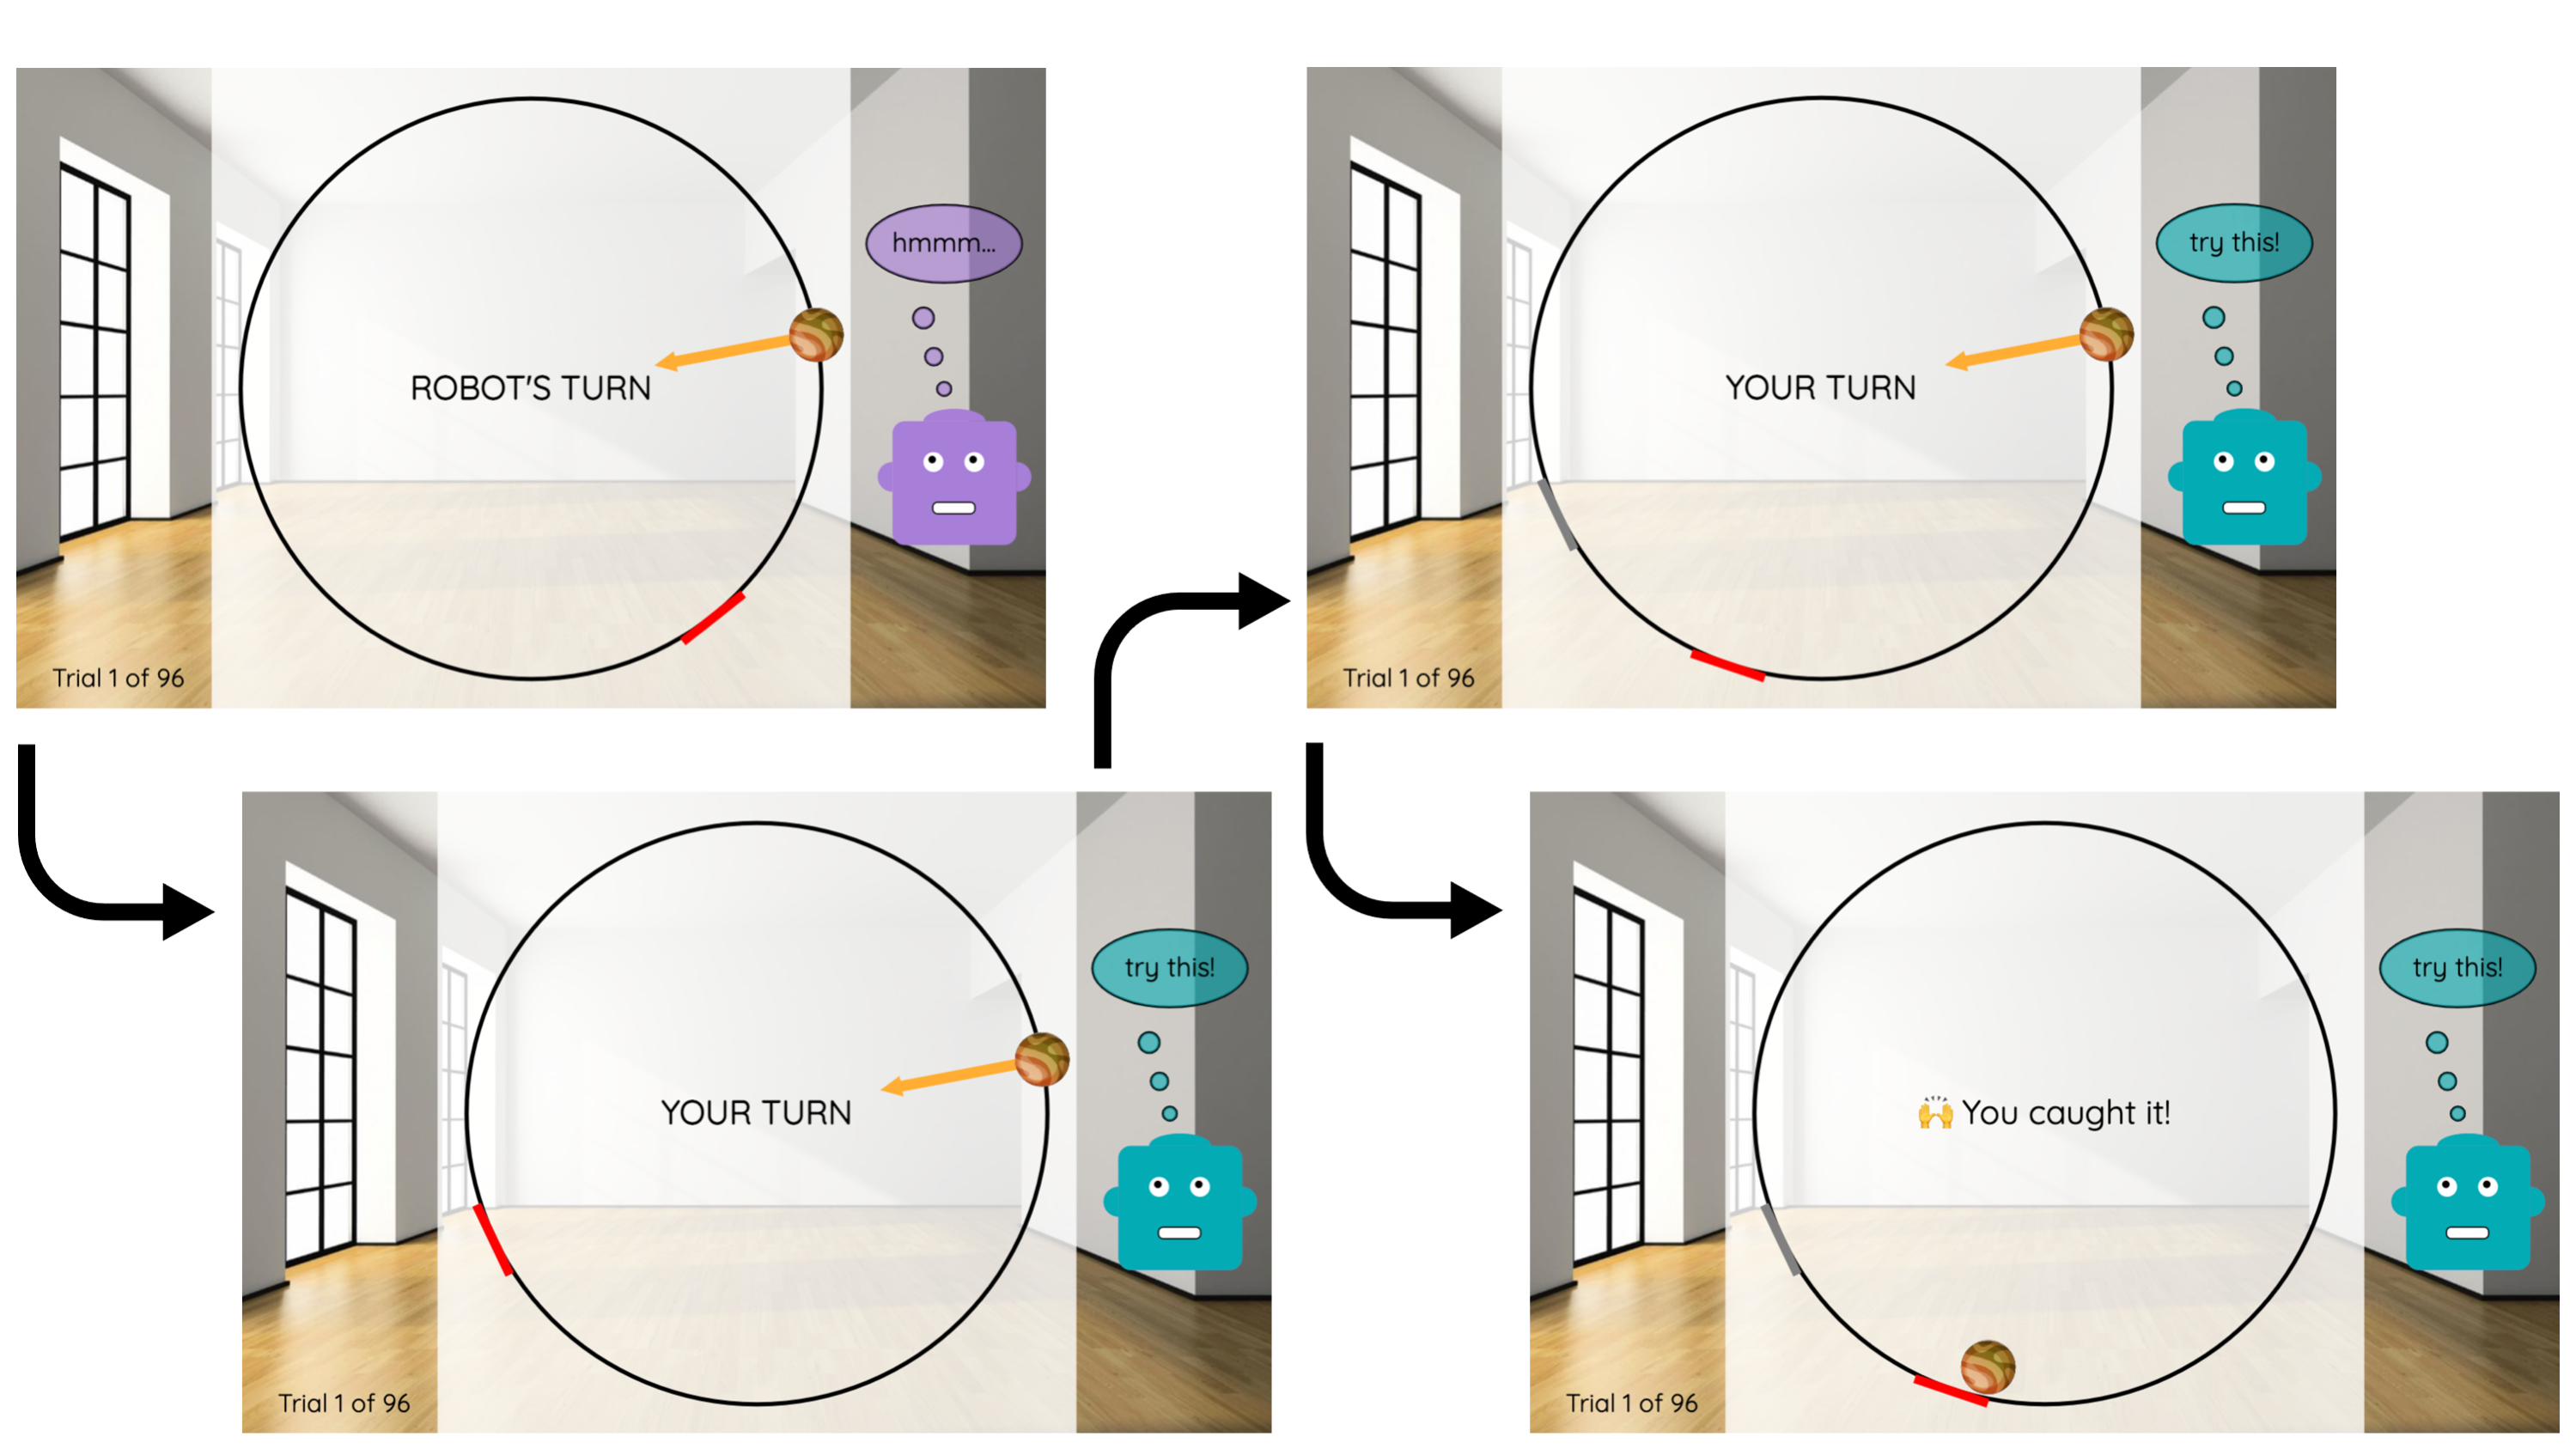
\includegraphics[width=\linewidth]{img/stimulus_overview.png}
\end{center}
\caption{A sample experimental trial. Top left: the bot partner moves the paddle to a suggested location. Bottom left: participants are given a chance to either keep the bot partner's suggested location or adjust it. Top right: after adjusting the bot partner's suggested paddle location, participants see the bot's original suggestion for comparison. Bottom right: participants are shown the result after launching the ball.} 
\label{fig:stim}
\end{figure}


Participants were assigned to one of four conditions that manipulated the quality of the bot partner's suggested paddle locations. In the \textit{low competence} condition, the bot gave suggestions whose quality (i.e., proximity to the ball's true landing location) varied considerably across trials. In the \textit{high competence} condition, the bot's suggestions varied little and were almost always close to the ball's final landing location. In the \textit{learning} condition, the bot's suggestions began with an accuracy profile similar to the \textit{low competence} agent but every 12 trials, it improved in discrete increments so that in the final 12 trials, its accuracy was similar to the \textit{high competence} agent. Finally, in the symmetrical \textit{worsening} condition, the bot agent began performing similarly to the \textit{high competence} agent but by the final block, made suggestions similar to the \textit{low competence} agent.

In each trial, the bot's suggested paddle location was an angle $x$ sampled from a von Mises distribution (a normal distribution defined over angles around a circle) with mean $\mu$ equal to the ball's final landing angle $\rho$, and variance $\kappa$ set based on the bot's competence level. The \textit{high competence} agent had a low $\kappa$ value of XX, meaning that the sampled paddle location was almost always close the ball's true landing location. In contrast, the \textit{low competence} agent sampled its paddle location each trial from a high variance distribution with $\kappa = XX$, meaning that while suggestions on some trials were accurate, many were not. The high and low competence $\kappa$ values were chosen to give the bots expected accuracy levels of around 80\% and 20\%, respectively. Meanwhile, the \textit{learning} agent began with a $\kappa$ value equal to the \textit{low competence} agent's $\kappa$ value, but every 12 trials the $\kappa$ was increased by a fixed amount so that in the final 12 trials, it had a $\kappa$ equal to the \textit{high competence} agent. The \textit{worsening} agent was symmetrical but in the opposite direction.

The task was composed of 96 trials divided into eight blocks of 12. These ``blocks'' were not visible to participants; in each block of trials, the ball appeared at a location sampled from each of the 12 hours on a clock face with some jitter so that participants would not rely on regularity in ball launch locations. The trials were randomized in each block so there was no structured pattern from one launch location to the next. The blocks were also used to update the accuracy of the \textit{learning} and \textit{worsening} agents described above; within each block, they had a stable accuracy that was better (\textit{learning}) or worse (\textit{worsening}) than the previous block. The ball's launching locations for the 96 trials were pre-computed to allow for simulations that calculated the ball's final landing location (they were therefore the same for every participant). However, the bot agents' suggested paddle locations were sampled during each trial as described above, allowing them to vary across participants. 

In each trial, we measured the bot's suggested paddle location, whether the participant chose to intervene or not, how far they moved the paddle, and whether they subsequently caught the ball. Overall, we hypothesized that people would use their own intuitive physics knowledge to coordinate with the bot agent, intervening more when the agent was more inaccurate and less when the agent was more accurate; we further hypothesized that people's intervention behavior would show sensitivity to the changes in competence demonstrated by the \textit{learning} and \textit{worsening} agents. However, a key additional hypothesis was that people would not make their intervention decisions in a vacuum, but would instead factor in their partner's past behavior when deciding whether they should intervene and how much. To test this, a randomly chosen trial in each block was designated as a \textit{critical trial}; rather than sampling the bot's suggested location as described above, the suggested paddle location on critical trials was chosen to have a fixed distance from the ball's estimated landing location. This distance (0.28 radians) was chosen to ensure that the agent's suggestion would not catch the ball, but would be close enough that a trusting participant might accept it. Each participant saw eight critical trials over the course of the experiment. We compare intervention behavior across conditions on these trials to see whether decisions about when to intervene and how much differed with each of the four bot partners even when the absolute error of the paddle suggestion was the same. 


\subsection{Procedure}

Participants were first shown a brief set of instructions outlining the task. They then completed 96 trials with their bot partner. Each trial began with the bot suggesting a paddle location that would catch the ball; the paddle was shown moving around the circle and a small animation on the right showed the bot ``thinking.'' Text in the middle of the circle read ``ROBOT'S TURN'' and during this time, participants' keyboard responses were disabled. Once the bot had moved the paddle to its suggested location, the animation concluded and the bot changed colors. Text in the center read ``YOUR TURN'' and participants were given the opportunity to either adjust the paddle's location with the arrow keys or simply keep the bot's suggested location. If participants adjusted the paddle location, the bot's original suggestion was indicated with a gray outline so that participants would be able to see how close the ball landed to the bot's original suggestion on each trial. When participants were happy with the paddle's location, they launched the ball using the spacebar (as soon as the ball was launched, they could no longer adjust the paddle location). The ball's launch trajectory was animated falling towards the paddle. If the ball made contact with any part of the paddle, this was considered a success. When participants successfully caught the ball, its location on the paddle was frozen and a message in the circle indicated that they had succeeded. If participants failed to catch the ball, it was shown falling out of the circle and a message in the center indicated that they had missed. Participants then pressed the spacebar to proceed to the next trial. 

After completing all 96 trials, participants were given a post-experiment questionnaire containing two parts. First, a series of demographic questions prompted participants for their age, gender identity (optional), level of education, and two covariates which we did not analyze here: number of physics classes taken in their life and hours of video games played in their life. Next, they were asked several questions about their decisions during the experiment. On a slider scale ranging from 0-100\%, participants indicated how often they thought they had intervened on the previous trials and how often they would expect to intervene if they were to play another 96 rounds with this same bot partner. Finally, they were asked to indicate on a five-point Likert scale how much they trusted the bot agent to catch the ball and how they decided whether to intervene on a given trial (two additional questions asked how much effort they had put into the task and whether they had experienced technical difficulties). 



\section{Results}

To understand how participants made the decision about whether to intervene or trust their bot partner, we compare three possible accounts of their decision making. First, it may be that people were entirely trusting of their bot partner, regardless of condition. On this view, we would expect no difference in intervention behavior across conditions and large differences in performance since the bots differed in their underlying accuracy. A second account takes the opposite perspective; instead, people may have essentially ignored their bot partner's suggestions, simply looking for the best paddle location each round (i.e., if the bot partner's suggestion was accurate, people would accept it and if not, they would intervene to correct it). Finally, a third possible account is that people's behavior was somewhere in the middle of these two. Rather than constantly following their bot partner's suggestion or unilaterally choosing the optimal paddle position each round, people may have relied on a combination of their own physical intuitions and the credibility or trustworthiness of their bot partner. [TODO say more here].

\subsection{People succeeded despite differences in bot partner ability}

We first ask whether there were any differences in people's overall ability to perform the task with each of the four bot partners. If people were entirely trusting of their partner's paddle suggestions or were unable to bring their own intuitive physics understanding to bear on the task, this would preclude the possibility that their collaborative decisions reflected nuanced judgments about their partner's competence. To understand how well people performed on the task with each bot partner, we look at how often they were able to catch the ball over the course of the experiment (\textit{accuracy}) and how far their final paddle location was from the ball's ultimate landing position (\textit{error}). Figure \ref{fig:results_summary} shows the average proportion of trials in which participants successfully caught the ball in each trial block across the four conditions (top left). Initially, accuracy was low for the \textit{low competence} and \textit{learning} agent conditions, presumably reflecting the fact that the bot partners gave poor paddle suggestions; participants would have faced low accuracy when trusting their partner and would have had to figure out the mechanics of the task themselves when intervening. In contrast, accuracy was high (between 70 and 80\%) in the \textit{high competence} and \textit{worsening} agent conditions. However, by the end of the experiment, participants all four conditions showed similarly high accuracy, suggesting that they were able to master the task in a way that was aligned with their partner's ability. The bottom left graph in Figure \ref{fig:results_summary} tells a similar story. Average distance of the paddle's center from the location where the ball crossed the circle (error in radians) was initially high for participants in the \textit{low competence} and \textit{learning} conditions but very quickly dropped in subsequent trial blocks and was similarly low across all four conditions by the end of the 96 trials. Broadly, this suggests that while people may have struggled to learn the mechanics of the task when their partner gave inaccurate suggestions, participants in all four groups developed a similar ability to perform the task with their bot partners. 


% FIGURE: Results summary
\begin{figure}[H]
\begin{center}
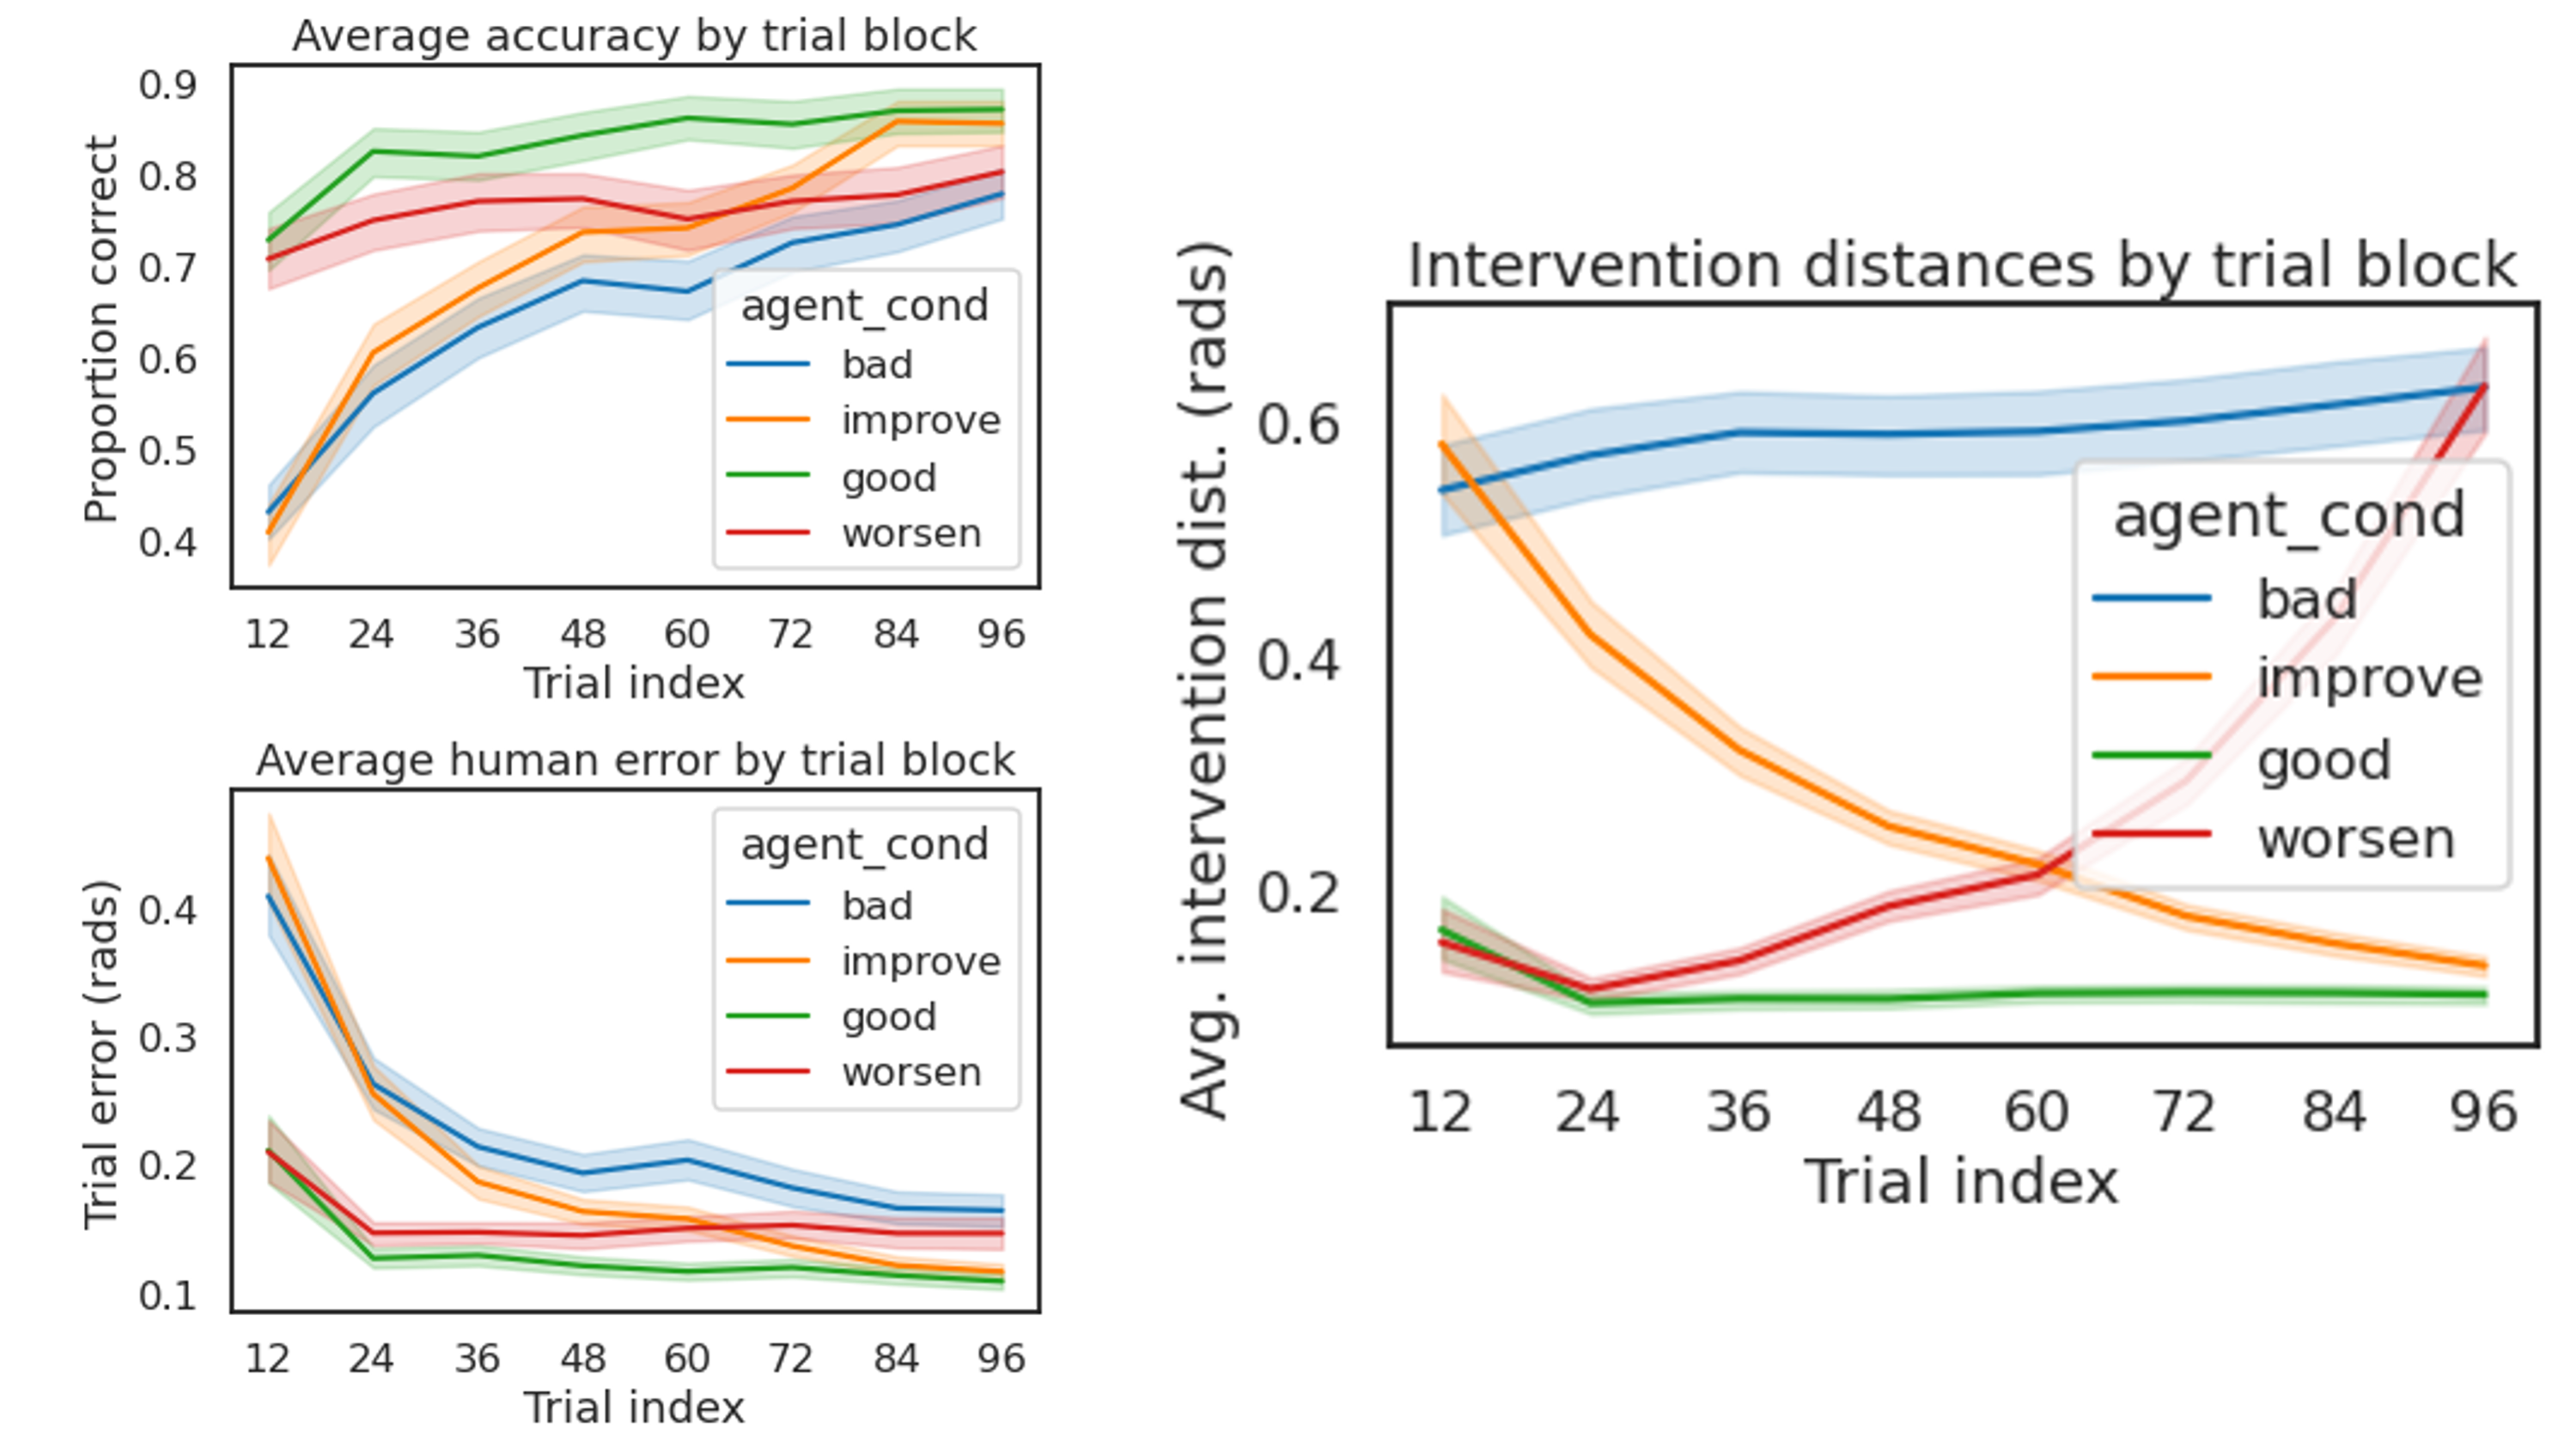
\includegraphics[width=\linewidth]{img/results-summary.png}
\end{center}
\caption{Summary of human-bot performance across conditions. Top left: average accuracy (i.e., whether participants caught the ball or not) by trial block across each of the four conditions. Bottom left: average error distance in radians by trial block across each of the four conditions. Right: average intervention distance by trial block in each condition. Overall, participants showed an ability to work successfully alongside their bot partner in all four conditions and their intervention behavior was calibrated to their partner's competence.} 
\label{fig:results_summary}
\end{figure}


The high accuracy level that participants eventually obtained with all four bot partners suggests that their intervention responses were calibrated to the bot's underlying competence. In other words, accurate and low-error responding would have looked very different across the four conditions. With the \textit{high competence} bot partner, participants could achieve high rates of success through minimal intervention, while success in the \textit{low competence} condition necessitated greater and more frequent intervention. Perhaps most interestingly, success with the \textit{learning} and \textit{worsening} agents would have required that participants be sensitive to the changing accuracy of their partner's suggestions. The graph at right in Figure \ref{fig:results_summary} shows average intervention distance (i.e., the average distance in radians between participants' final paddle placement and their bot partner's initial suggestion) in each trial block across the four conditions. Consistent with the hypothesis above, intervention distances were highly calibrated to the bot partner's ability across the four conditions, with large intervention distances in the \textit{low competence} condition, small intervention distances in the \textit{high competence} condition, and intervention distances that roughly tracked the accuracy changes of the \textit{learning} and \textit{worsening} agents. This latter result suggests that people did not regard their bot partner's ability as \textit{static}, instead calibrating their responses to improvement and decline in the bot's accuracy. Thus, the results in Figure \ref{fig:results_summary} indicate that participants succeeded in collaborating with their bot partner on the task and did so by calibrating their interventions to their partner's underlying accuracy.


\subsection{People trusted bot partners}

Given participants' successful calibration to their bot partner over the course of the experiment, one account of people's behavior in the task is that they simply relied on their own intuitive physics model to respond. This internal model may have been poor at first, leading to lower initial accuracy for participants in the \textit{low competence} and \textit{learning} conditions. Critically, on this view, their partner's ability is essentially irrelevant; given the ball's starting location, participants estimated its final landing point and moved the paddle there if it needed to be moved or left it if not. If this were true, then there would be no evidence of \textit{trust} in people's behavior, e.g., minimal adjustments in the \textit{high competence} condition would simply reflect the fact that on most trials, little adjustment was needed (and vice versa for the \textit{low competence} agent). 

However, another possibility is that people maintain an ongoing latent estimate of their partner's ability and this estimate \textit{informs their intervention behavior}. In other words, in the \textit{high competence} condition, participants balance their own estimate of where the paddle should be with the fact that they expect their partner's estimate to be pretty good. Meanwhile, in the \textit{low competence} condition, participants are accustomed to making large interventions on behalf of their partner and therefore place less confidence in their partner's estimates even when they are fairly accurate. This latter view offers a basic operationalization of participants' trust in their partner.

To test these two hypotheses, we compare intervention behavior on the eight \textit{critical trials} that participants saw over the course of the experiment. If people's responses were merely a result of estimating the ball's final location and placing the paddle there, we should not see any difference between the four conditions on these trials, since the amount they would have to intervene was identical. However, if people's behavior in part reflected an underlying judgment about their bot partner's credibility or trustworthiness, then we might expect their intervention decisions to differ across the four conditions. Figure \ref{fig:critical_trials} shows participants' average intervention rates on critical trials (i.e., the proportion of critical trials on which they intervened) and the average intervention distance (i.e., how far they moved the paddle from its suggested location) across the four conditions. First, while intervention rates were relatively high on critical trials overall, participants in the \textit{high competence} and \textit{worsening} conditions were less likely to intervene on these trials than those paired with \textit{low competence} and \textit{learning} partners. This suggests that people's decisions about whether it was necessary to intervene on critical trials were influenced by the initial competence of their partner. Second, people showed a similar but even more dramatic pattern in their intervention distances on critical trials. While those paired with a \textit{low competence} or \textit{learning} bot partner adjusted the paddle by an amount close to the optimal level of 0.28 radians on average, participants whose partner was very accurate (\textit{high competence}) or started out highly accurate (\textit{worsening}) made significantly smaller adjustments on critical trials. Thus, a complete account of  reasoning on this task is not limited to participants placing the paddle in the best possible location on each trial, but rather, factoring an underlying assessment of their partner's competence into the decision about whether to intervene and how much.


% FIGURE: Critical trials
\begin{figure}[H]
\begin{center}
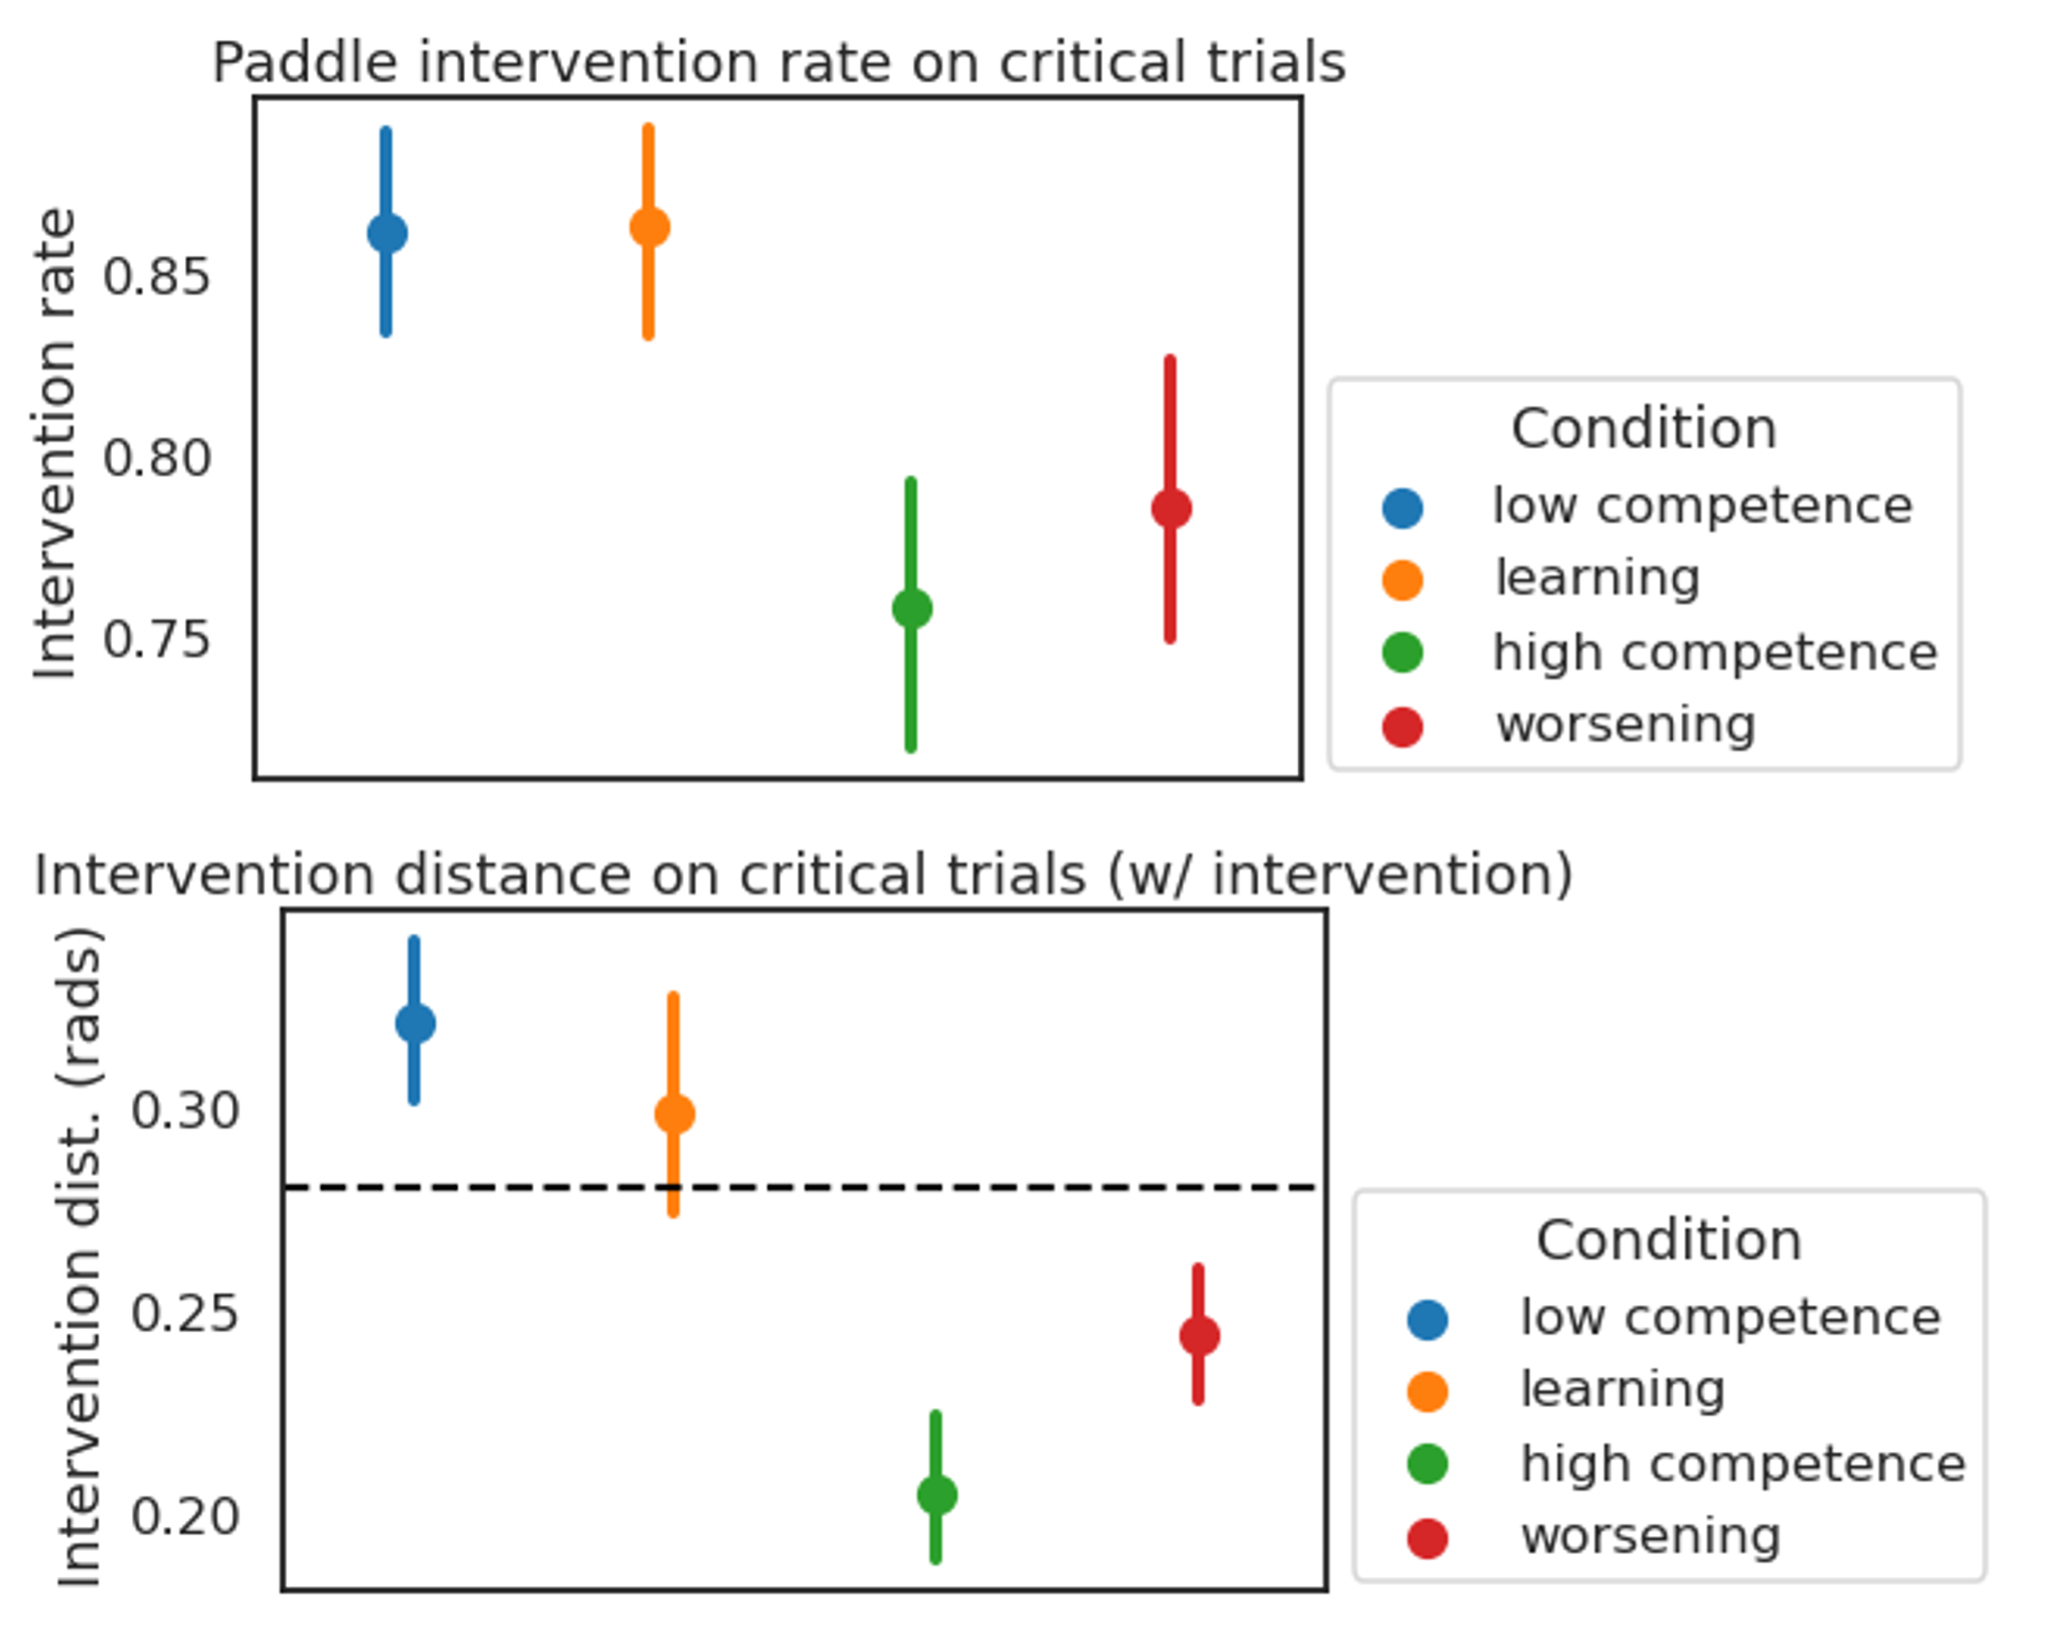
\includegraphics[width=\linewidth]{img/results-critical_trials.png}
\end{center}
\caption{Intervention behavior on \textit{critical trials}. Left: average proportion of critical trials on which participants chose to intervene. Right: average distance participants intervened on critical trials. The dashed line indicates the optimal intervention distance on these trials. Even though the bot partner's suggested paddle location was the same distance from the ball's landing point on all critical trials, participant responses were sensitive to their partner's competence, intervening less when their partner was initially accurate.} 
\label{fig:critical_trials}
\end{figure}


\subsection{OPTIONAL: post-survey results}



\section{Discussion}



% \section{Acknowledgments}
% In the \textbf{initial submission}, please \textbf{do not include
%   acknowledgements}, to preserve anonymity.  In the \textbf{final submission},
% place acknowledgments (including funding information) in a section \textbf{at
% the end of the paper}.





\bibliographystyle{apacite}
\setlength{\bibleftmargin}{.125in}
\setlength{\bibindent}{-\bibleftmargin}
\typeout{} % erikb for some reason this line is necessary...
\bibliography{references}


\end{document}
